\section{Use of the Operators in a Surveillance Camera System}


To coordinate these models, we specify how the previous operators are applied by defining a \bflow specification (see Listing~\ref{lst:bflowcamerasystem}). To coordinate the activity BatteryControl and the TFSM CameraControl, we have to apply the operator SyncFSMEventsAndActions that synchronizes the corresponding Action and FSMEvent by relying on theirs names (Listing~\ref{lst:bflowcamerasystem}: line 8). Then, we have to specify a timing and hierarchical coordination between the states of the TFSM CameraControl and the activities doJPEG and doJPEG2000. To express that, we have to specify that the operators startActivityWhenEnter and AtomicActivity must be applied between the TFSM CameraControl and each activity (Listing~\ref{lst:bflowcamerasystem}: line 9 to 12).

In the modeling workbench, we use the \bflow specification to generate the model of coordination that results in six \ccsl relations. Then, we use the modeling workbench to execute the \ccsl specification of the surveillance camera system. Figure~\ref{fig:camerasystem} illustrates the partial timing output of the execution of the camera. The \mse FSMEvent \emph{BatteryisHigh:occurs} and the Action \emph{BatteryisHigh:executeIt} result strongly synchronized (in red in Figure~\ref{fig:camerasystem}). When the camera is in BatteryHigh state (in magenta in Figure~\ref{fig:camerasystem}), the activity is allowed to execute (in cyan in Figure~\ref{fig:camerasystem}). During the execution of the activity, the time in the TFSM does not elapse. This results in no occurrences of the \mse \emph{ms:ticks}.
	
The complete example can be found in the companion website that contains the models together with a detailed procedure to execute and verify them. In addition, the site includes a video that shows the complete workflow by using the GEMOC studio. 
%the operator SyncProdut must be applied one time to coordinate the models … Then, the operators startActivityWhenEnter and AtomicActivity must be applied twice, one time for each activity. This specification is only for one camera which is composed by three models. However, this can be extended for N camera by modifying the bflow. 
		\begin{figure}
			\center
			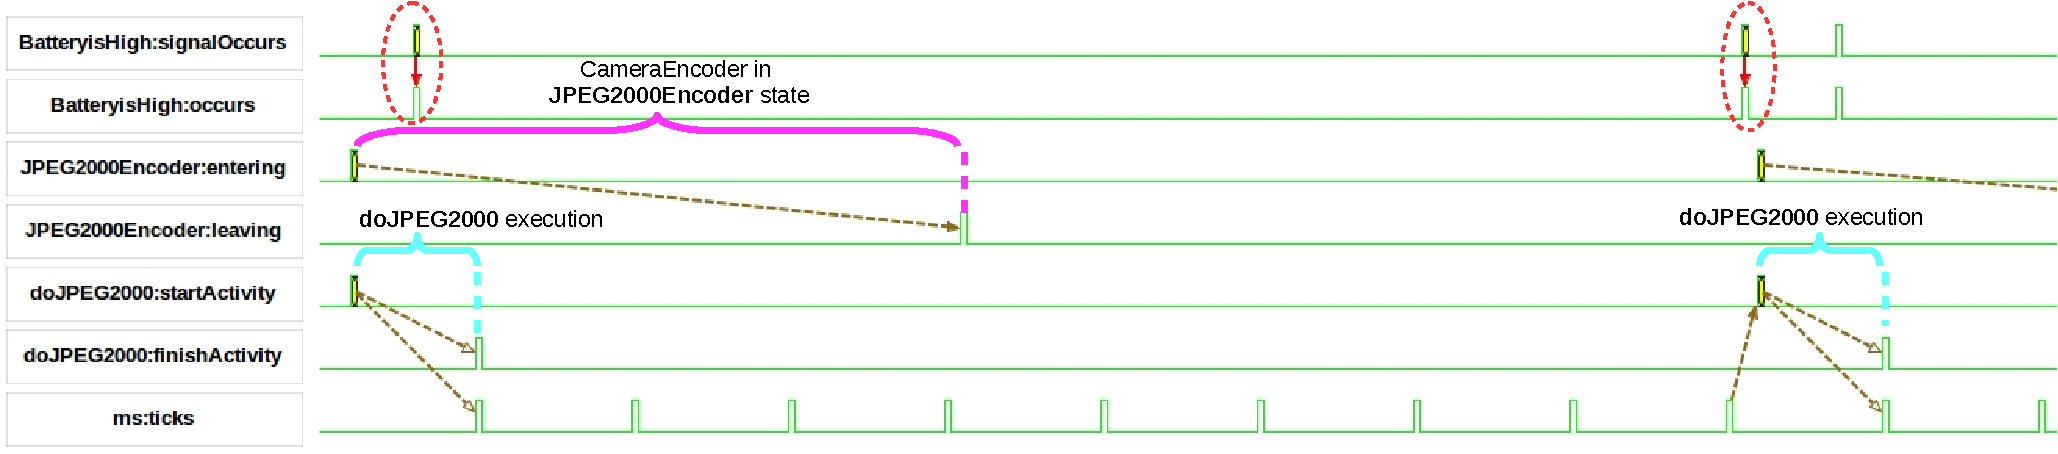
\includegraphics[width=1\columnwidth]{examples/figs/vcdcamera}
			\caption{Resulting timing output of the surveillance camera system}
			\label{fig:camerasystem}
		\end{figure}
	
	
	
		\begin{lstlisting}[language=bflow,
		caption={\bflow specification for the Surveillance Camera System},
		label={lst:bflowcamerasystem}, 
		basicstyle=\scriptsize\ttfamily, backgroundcolor=\color{LGrey}, numbers=left, xleftmargin=2pt]
		BCOoLFlow CameraSystem
		ImportBCOoL  "TFSMAndActivityHierarchical.bcool" ;
		Model BatteryControl "batterycontrol.ad"
		Model CameraControl "cameracontrol.tfsm"
		Model doJPEG "doJPEGAlgorithm.ad"
		Model doJPEG2000 "doJPEG2000.ad"
		Flow 
			applies SyncFSMEventsAndActions between (BatteryControl, CameraControl);
			applies startActivityWhenEnter between (CameraControl, doJPEG);
			applies startActivityWhenEnter between (CameraControl, doJPEG2000);
			applies AtomicActivity between (CameraControl, doJPEG);		
			applies AtomicActivity between (CameraControl, doJPEG2000);		
		end Flow;
		\end{lstlisting}